\documentclass[12pt,a4paper]{report}
\usepackage{graphicx} 
\usepackage{fancyhdr}
\pagestyle{fancy}
\usepackage{fontenc}
\usepackage{url}
\usepackage{float}
\usepackage{lastpage}
\usepackage[utf8]{inputenc} 
\usepackage{polski} 
\author{Michał Jendraszczyk}
\begin{document}
\lhead{Amnesia - Advena}
\rhead{}
\linespread{1.3}
\title{\textbf{\huge{Amnesia - Advena}} \linebreak \large{Gdzieś pośród setek wspomnień...}}

\begin{titlepage}
  \thispagestyle{plain}
 \thispagestyle{empty}
  \maketitle 
\end{titlepage}

\pagebreak  
\tableofcontents
\pagebreak 
\section{\textbf{Prolog}}
\subsection{Gorzkie wspomnienia}
\begin{center}
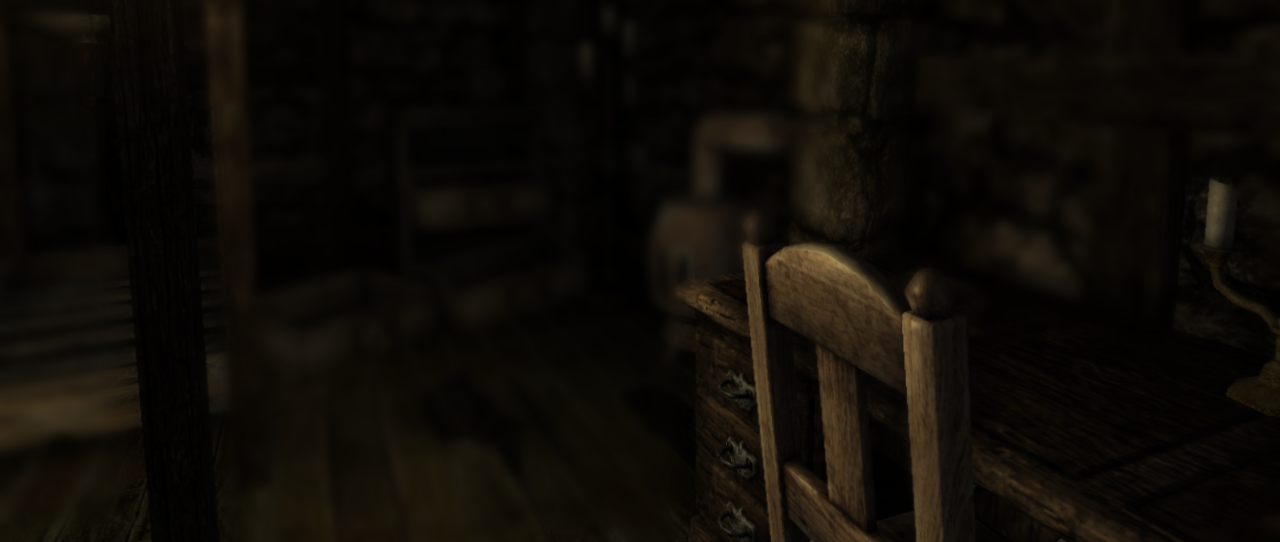
\includegraphics[scale=0.31]{C:/Users/Tasjen/Pictures/AMNESIA_SCREENS/r1.png} \\
\end{center} 

Kolejna burzowa noc na mym dziedzińcu i zarazem kolejna okazja na chwilę refleksji. Chociaż, nie sądzę, aby był na to dobry moment, kiedy to moją jakże krótką egzystencje przepełnia grom nieszczęść. Lada dzień a dane mi będzie gościć w mych progach moich najbliższych z okazji moich urodzin, lecz cóż to właściwie zmieni w moim życiu? - W jaki sposób ta chwila sztucznej euforii wywołanej jakby z poczucia konserwatywnych zasad miała wpłynąć na ucieczkę od przeszłości. Minęła już dobre ćwierćwiecza odkąd to się stało – a cały czas mam ten obraz uchodzących wspomnień niczym miałoby to miejsce ledwie wczoraj. Każdej nocy sen przerywa mi koszmar widoku brutalnie gwałconej żony, która z poderżniętymi ścięgnami stóp świadomie czekała na swój koniec. Nie próbowała nawet stawiać oporu, widząc porozrzucane po komnacie wykrwawione już zwłoki ledwie kilku letnich dzieci. A ja... - Ja nie mogłem zrobić z tym nic. Kompletnie nic. Czemu więc kiedy mnie zobaczył popełnił samobójstwo? Zemsta? – Zazdrość? – Czymże oni wadzili i komu, za co zasługiwaliby na taki koniec? - Nie wiem...   I prawdopodobnie nigdy się już nie dowiem. Nie miałem okazji nawet wymierzyć sprawiedliwości, która ku głębszemu zastanowieniu nie byłaby nawet w najmniejszym stopniu miarodajna w stosunku do tego, co dotknęło mnie... Gdzie w jednej chwili straciłem całe życie...
 
\subsection{Prace remontowe}

Muszę przyznać, że im dłużej piszę, tym rzadziej mam ochotę sięgać po pióro. Tę późną wiosną postanowiłem poświęcić czas na drobny remont w moich apartamentów Rozkazałem, więc bez dwóch zdań swoim lokajom, aby zabrali się w końcu za tą wiecznie psującą się kanalizę, której ulatujący smród wprost nie daje mi spokojnie spać po nocach. Jeden z inżynierów – Aleppo\footnote{Aleppo - magister inżynier budownictwa z specjalizacją  inżynierii hydraulicznej, zajmujący się naprawą kanalizy możnowładcy}  - postanowił zorganizować ekipę pracowników, która zajmie się problemem, bezpośrednio - u źródła. Kiedy już prace ruszyły pełną parą – ciężko było znaleźć chwilę spokoju, którego przez wzgląd na mój charakter potrzebowałem najbardziej, dlatego też głównie przesiadywałem w prywatnej bibliotece studiując tam zawarte mądrości. Pewnego wczesnego, ledwie przedpołudnia jeden z pracowników zajmujących się tym śmierdzącym defektem – poinformował mnie o tajemniczym odkryciu na terenie mojej posiadłości. Nieco zirytowany tą sytuacją kazałem temu łachudrakowi wynosić się, czym prędzej z mojego pokoju i wracać, czym prędzej do roboty. On jednak nalegał abym zobaczył to coś, co według niego – tego prostego człowieka było czymś zupełnie obcym. Eh, zagroziłem temu skamlającemu mi nad tyłkiem psu, że jeśli jest to coś mało interesującego – natychmiast ląduje na zbity pysk, nie dostając za robotę złamanego grosza. Facet mimo to nie odstępował od swoich słów, a więc zdążyłem się poświęcić na taplanie się w gównie. Razem z nim udałem się do reszty ekipa, która była zszokowana tym, co ujrzeli. Podczas prac remontowych w kanale znaleziona została ukryta komnata. Niby nic dziwnego, gdyby ją jednak nie okalały jakieś dziwne znaki i przedziwna księga, na której wygrawerowany był napis Annimus – Advena \footnote{Annimus Advena - księga opisująca metody transfmutacyjne istot żywych.} . Rozkazałem ludziom zaprzestać prac drenażowych i skupić się na eksploracji tej komnaty w poszukiwaniu znalezisk, jakie w sobie kryje – oczywiście wszystko to za podyktowaną podwójną zapłatą. W momencie, kiedy reszta zajęła się pracą, ja tymczasem zabrałem znalezisko do swej biblioteki by móc przyjrzeć się temu bliżej.
 
\subsection{Księga Annimus - Advena}

 
Po niespełna miesiącu – po kilkuset godzinach spędzonych na analizie zawartych w Advena – Annimus – w końcu znalazłem jej sens. Ta księga ewidentnie zawiera w sobie niezbadane runy, które prawdopodobnie pozwalają na manipulację pierwiastkami życia i śmierci. Jego inteligencja podpowiadała mu, że jedynym sposobem na opanowanie tajników zawartych w księdze jest przeprowadzanie badań na żywym ciele. Z tego też powodu, dosyć lekkomyślnie podjął się brutalnych metod w imię nauki. Przy pomocy moich podwładnych ściągałem świeży materiał do badań. Idealnie przydał się do tego karcer, który przebudowany został z jeszcze niedawnych piwnic.  Moi dawcy prawdopodobnie w chwili trafienia tutaj nie mieli do tej pory bladego pojęcia – po co i dlaczego zostali tu sprowadzeni, jednak – ta świadomość, nie miała tu większego znaczenia. Ich los był już z góry przesądzony. Kiedy prace nie przynosiły większych efektów, a materiał do badań nieubłaganie się kończył zmuszony byłem uszczuplić nieco moją kadrę pracowników. Niestety – jednak zamiast oczekiwanych rezultatów otrzymywałem przerażające twory, których widok paraliżuje moje ciało i umysł. Te ohydne stwory stawały się jakby mrocznymi cieniami pierwotnych istot. Swoje pseudo eksperymenty przeprowadzałem w podziemnych kazamatach starając się, aby nie ujrzały światła dziennego.
 
\subsection{Eksperyment}
 
Celem, jaki sobie postawiłem jest może nieco irracjonalna, ale jedyna możliwość wpłynięcia na tragiczny los z przeszłości, który z wielkim smutkiem dźwigam niczym brzemię. Wierzę, że z pomocą nauki uda mi się przetransferować duszę w inny wymiar, jednak potrzebuję do tego ofiary.  Nie bacząc na los niewinnych, poświęconych istot ludzkich, zapominając o konsekwencjach swoich czynów – po trupach szedłem do celu. W końcu - nadszedł moment przeprowadzenia badań na swojej osobie. Jestem pewien, że nie będzie innego już drugiej takiej okazji. Muszę spróbować ocalić rodzinę.... Już wszystko gotowe.... Czuję, jak ulatuje mi resztka martwych wspomnień. Czuję, że... Ja... - Cholera – gdzie ja jestem! – Kim lub czym jestem? – I co ja tu robię...?!
 
\subsection{Blask nadziei}

Myśląc, że me oczy już na zawsze pochłonął mrok, po długim czasie nagle ujrzały światło. Nie mogąc zasięgnąć do wydarzeń z przeszłości, jak gdyby zły los nie pozwolił mi po nie sięgnąć obudziłem się w przegniłej komnacie pełnej kurzu, pajęczyn i ludzkich kości. Nie wiem co za ciemne moce sprowadziły mnie w to przeklęte miejsce, ale już w pierwszych krokach po niczym skutej lodem posadzce zaczęły dopadać mnie dziwne dreszcze. Otoczyła mnie aura niepokoju jednak nieświadomość sytuacji w jakiej się znajdowałem, a z drugiej strony nadzieja na powodzenie eksperymentu pozwoliła mi wykonać kolejny krok, krok który rozświetlił w moim umyśle dalszy sens moich poczynań.   
 
\section{\textbf{Rozdział 1}}
\subsection{Kazamaty Issac'a}
\begin{center}
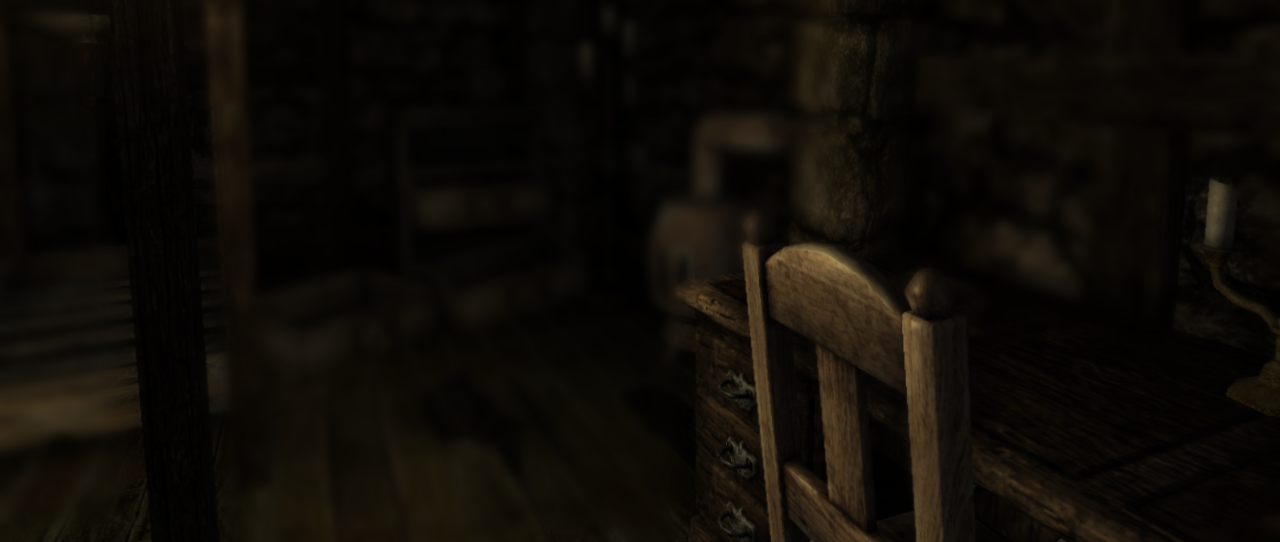
\includegraphics[scale=0.31]{C:/Users/Tasjen/Pictures/AMNESIA_SCREENS/r1.png}\\
\end{center}

Idąc wgłąb podziemnych korytarzy zacząłem zdawać sobie sprawę, jakbym te ściany, ta podłoga, regały, i naczynia w dziwny nie były mi obce. Czyżbym znał to miejsce? A może to po prostu wytwór mojej wyobraźni? Może to tylko sen? Sen na jawie... Stąd też zdaje mi się słyszeć skowyt bestii, jęki konających i ten szelest nietoperzy okalający całą sieć pomieszczeń. Jednak nie stanowiło to dla mnie żadnego dyskomfortu. Nie czułem strachu, bo dlaczego miałbym go mieć, skoro nie mogłem już nic stracić. Kiedy dokładniej zacząłem eksploatować okolicę co jakiś czas znajdywałem fragmenty pergaminu opisującego zdarzenia z całkiem nieodległej przeszłości. To dziwne, ale mam przeczucie jakoby miało to ze mną związek. Postanowiłem zbierać te fragmenty i czas pokaże, może uda mi się znaleźć okoliczności w jakich tu się znalazłem. Czytając znalezione tu manuskrypty dowiedziałem się, że miejsce to jakieś mroczne kazamaty, które okala niezbyt przyjemna historia. Te ściany komnaty dotknęło niejedno ludzkie cierpienie. Zauważyłem nadto, schody prowadzące w dół do jakiegoś starego karcera\footnote{Karcer - miejsce przetrzymywania ofiar poddawanych pseudo eksperymentom} . Prawdopodobnie już nie funkcjonującego, ale kto wie, może i tam znajdę jakieś wskazówki. W środku zastały mnie przeszywające jęki umęczonych dusz oraz dziwny chłód, którego nie jestem w stanie opisać. Czyżby ten loch był nawiedzony? Co przyjdzie mi tu jeszcze spotkać nim skonam ze strachu. Idąc niepewnym krokiem wzdłuż upiornego korytarza, przylepiony do ściany, dzięki której mogłem w jakiś sposób zorientować się w terenie, nagle usłyszałem głos. Mój stan psychiczny był na tyle już słaby, że nie byłem już do końca pewien czy to rzeczywiście usłyszałem, czy może był to po prostu wytwór mojej wyobraźni. Lekceważąc to usłyszałem ponowne wołanie. Zapytałem się kto lub co mnie wzywa i w jakim celu, w końcu nikomu nie zawiniłem. Postać z mroku odpowiedziała konającym głosem, że nie chce ginąć w głodowych męczarniach. Postanowiłem mu w jakiś sposób pomóc, zszedłem w dół do spiżarki i przyniosłem kawałek czerstwego chleba. Obcy przedstawił mi się jako Zikvin\footnote{Zikvin - jeden z więźniów, któremu decydujemy się pomóc, będący niegdyś jednym z lokajów możnowładcy} . Był niegdyś jednym z członków lojalnej służby domowej, jednak niedoceniony przez Pana, trafił w oblicze jego mrocznego eksperymentu. Więzień w wyrazach wdzięczności podarował mi fragment magicznego kryształu. Jeszcze nie wiem po co mi coś takiego, ale niekulturalnie byłoby odmawiać podarunku. Badając więzienne komnaty natknąłem się kolejny fragment jakiegoś pamiętnika. Po przeczytaniu ni stąd ni zowąd mym oczom ukazało się straszydło. Jego ciało wskazywało by na cechy ghula i zombie. To musiał być cadavr\footnote{Cadavr - mutacja ghula z zombie, za pomocą zmysłu węchu i słuchu jest w stanie błyskawicznie zlokalizować przeciwnika atakując go przeszywającymi do szpiku kości szponami}  błąkający się po tutejszych komnatach. Martwa skóra przeszywana była przez żelazne łańcuchy jakimi obezwładniono go jeszcze za żywota, oczy, a w zasadzie ich brak powodowały u mnie zawroty kiedy tylko spojrzałem w jego stronę. Kiedy tylko jego postać znikła w mroku czym prędzej pognałem do wyjścia słysząc ciągle za sobą jej skowyt. Opuszczając karcer doszedłem do wniosku, że poszukać stałego źródła światła. Nie ma nic gorszego niż przeczesywanie chwiejnym krokiem ślepo podążając przed siebie. Podczas pobytu w tym upiornym miejscu na podstawie analiz zrozumiałem, że kluczem do wyjścia byłyby wodociągi, które jak przypuszczam w którymś korycie uchodzą na światło dzienne. Zardzewiały właz jednak ani drgnie, toteż począłem szukać innej, alternatywnej drogi lub wskazówki, która przyczyniłaby się do osobistego sukcesu. Pośród otaczającego mnie smrodu, przesiąkniętym krwią drewnianym blatem ledwie stojącego stołu dostrzegłem jakby magiczną formułę, używaną do przyzywania istot z zaświatów. Nie zastanawiając się dłużej przeszedłem do sedna, mianowicie - składników niezbędnych do odprawienia rytuału. Według tego co było zapisane konieczna była limfa, szkielet, w którym mogłaby osadzić się istota oraz roztwór nerblantu\footnote{Nerblant - materiał będący spoiwem organów podczas rytuału przywołania istoty z zaświatów  } , będącego spoiwem zgromadzonych trofeów. W chwili wykonania rytuału w pustym laboratorium niczym zjawa ukazało mi się przerażające monstrum. Moja psychika tego nie wytrzymała. Gdy ocknąłem się byłem już zupełnie sam. Może był to kolejny koszmar? Może wszystko, co dotąd robię to zły sen z którego nie mogę się wybudzić? W takim razie może wystarczyłoby po prostu sobie pomóc. W jakiś sposób przyczynić się do załamania tej struktury? Pobiegłem więc w dół, nawet nie ruszyło mnie w żaden sposób to w jakim stanie znajdują się roztrzaskane drzwi, które jeszcze niedawno były szczelnie zamknięte. W kotłowni znalazłem zawór doprowadzający gaz do pieca. Odkręciłem go, chciałem wreszcie to skończyć. Skończyć ten mało śmieszny kabaret. Kiedy otworzyłem piec mym oczom ukazał się tajemniczy klucz. Może jednak jeszcze jest szansa? Tylko... Nagle coś buchnęło, zionęło, uderzyło. Wszystko zaczęło się walić, a cała kotłownia stanęła w płomieniach. Czyżby to jakaś kolejna niespodzianka mojego wytworu wyobraźni? Chociaż stale sobie to tłumacząc sytuacja ta była jak najbardziej rzeczywista, zarówno w przyczynie jak i skutku. To musiałbyś samozapłon w wyniku ulatniającego się gazu. Nie myśląc dłużej, pobiegłem przed siebie, przez płonące drewniane schody, zawalającą się tregrę, pośród pękających menzurek alkoholi i oliwy wzmagającej pożar. Dotarłszy na górę chwyciłem klucz, włożyłem go w zamek i lekko przekręciłem. Drzwi, które żadna siła nie była w stanie otworzyć, nagle jak na zawołanie stały przede mną otworem.  
 
\section{\textbf{Rozdział 2}}
\subsection{Wodociągi} 
\begin{center}
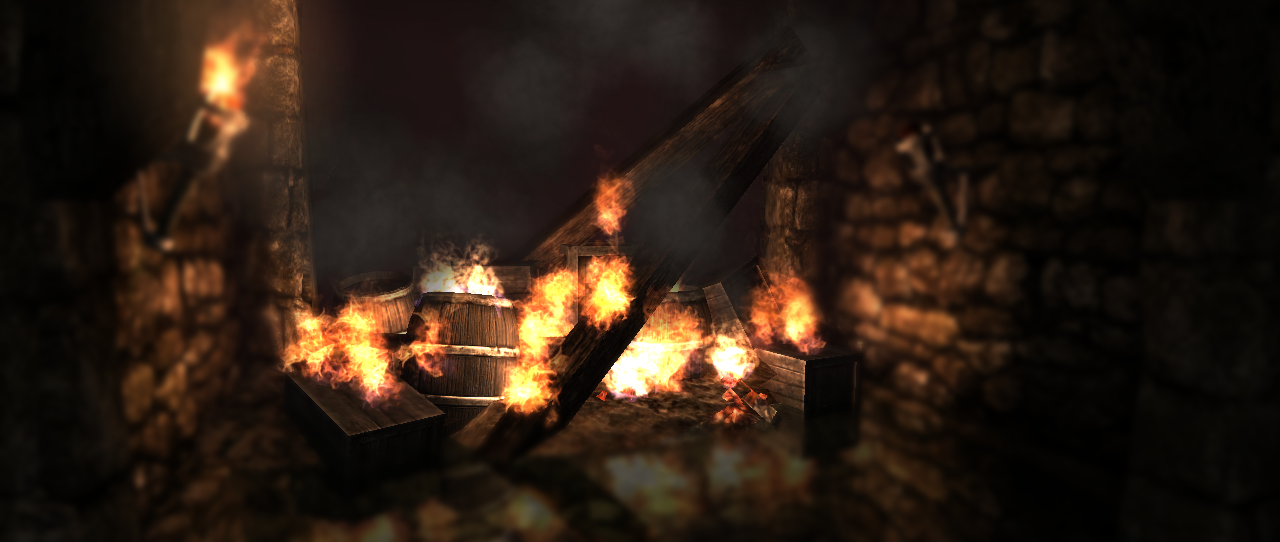
\includegraphics[scale=0.31]{C:/Users/Tasjen/Pictures/AMNESIA_SCREENS/r2.png} \\
\end{center}
 
Ledwie przekroczywszy próg wodociągów za moimi plecami rozległ się huk. Okazało się, że droga powrotna jest niemożliwa. Pozostało mi więc iść przed siebie. Kilka kroków dalej, idąc w zalanym po kolana korytarzu dostrzegłem stertę płonącego gruzu. Wiedziałem - nie było co się kusić, że dalej będzie z górki. Po lewo dostrzegłem wyrwę w ścianie prowadzącą do sąsiedniego przedsionka, jednak powstała awaria gazowa uniemożliwiła mi sprawdzenie tego miejsca. Nie mając możliwości powrotu, będąc odciętym ze wszystkich stron, szukałem sposobów na choćby najmniejszy postęp. W owym przedsionku, zaraz obok znajdował się magazynek. Nawilżyłem chustę w wodzie, a następnie czym prędzej pognałem przed siebie. Docierając na miejsce natychmiast zatrzasnąłem pewnie stojące w ościeżnicy, drzwi. Pośród setek skrzyń poczułem nagle jak coś spada mi na głowę. Chłodny, wilgotny, poranny deszcz ulatujący, jak by niepewnie z wyrwy w suficie będącego głęboko pod ziemią. Po chwili refleksji, dostrzegłem dobrej jakości, stalowe kolano $ \phi $ 32. Sądzę, że miał on tu posłużyć jako wymiennik w wypadku awarii instalacji. Korzystając z okazji, chwyciłem je i ruszyłem do pomieszczenia obok naprawić usterkę. Kilka obrotów wystarczyło aby uszczelnić instalację na tyle, aby móc dokładniej się rozejrzeć. Nad sufitem ujrzałem zwisający sznur prowadzący na górne piętro. To ciekawe, sam powróz przymocowany został do metalowej klapy sprawiającej wrażenie zaspawanej. Wdrapawszy się na górę, już wszystko zrozumiałem. Okazało się, że klapa jest możliwa do otworzenia z wykorzystaniem ciśnienia hydraulicznego regulowanego przez dźwignie otwierające zawory. Korzystając z zapisanych obok wskazówek przełączyłem w następujący sposób zawory, poprzez które wytworzone ciśnienie wyrwało ledwie trzymający się spaw blokujący zejście. 
\begin{figure}[H]
\begin{center}
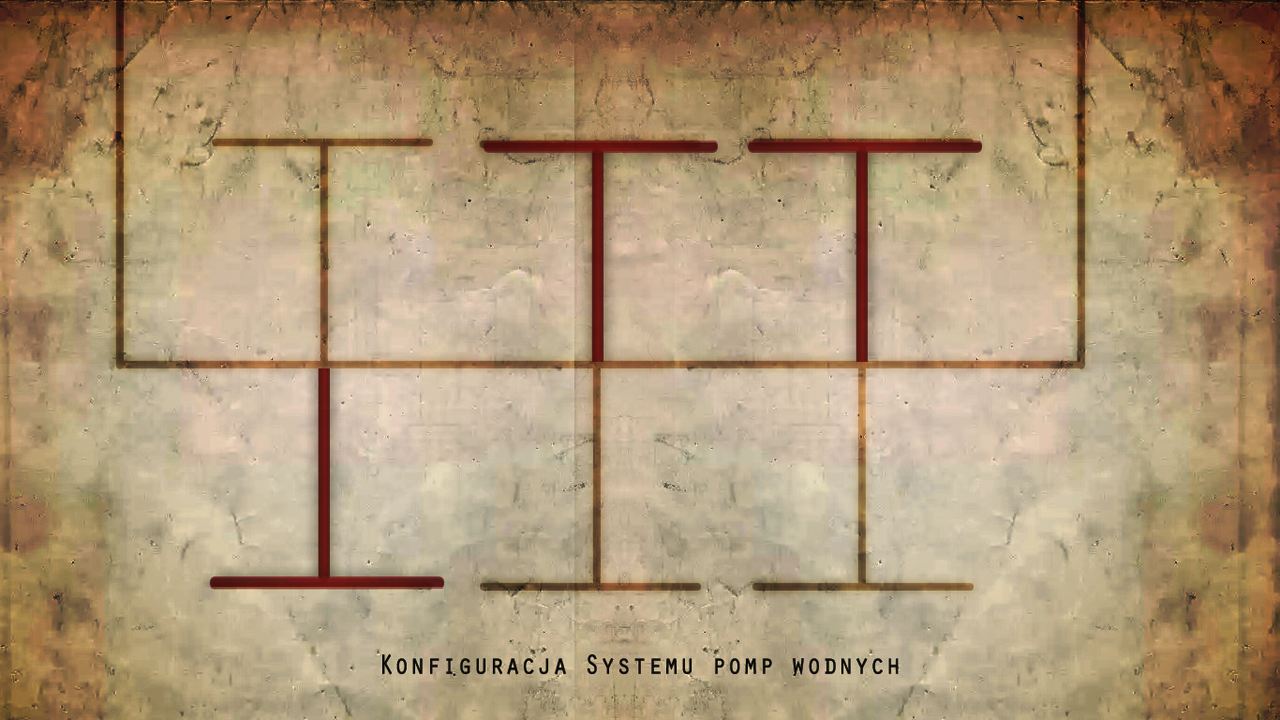
\includegraphics[scale=0.31]{C:/Users/Tasjen/Pictures/AMNESIA_SCREENS/amnesia_act1toact2.png} \\
\end{center}
\caption{Konfiguracja zaworów regulujących ciśnienie}
\end{figure}

Będąc na dole, coś zaczęło mnie gonić. Nie byłem w stanie ocenić co to w ogóle jest. W żaden sposób nie można było określić materii tego stworzenia. Ni to zjawa, ni duch. Jego środowiskiem egzystencjalnym stawała się być wyłącznie woda. Według przeanalizowanych niegdyś ksiąg stworzenia takie nazywano kurgarami\footnote{Kurgar - niematerialna istota żyjąca w środowisku wodnym, żywiąca się ludzkim mięsem.} . Ruszyłem ile sił w nogach przed siebie.  W trakcie ucieczki przed tym tworem wziąłem stojące obok kilkunastu litrowe drewniane wiadro. Pomyślałem że może się okazać przydatne w celu ugaszenia pożaru na górnym piętrze. Zapadła cisza. Siedząc nieruchomo na jednej z skrzyń potwór ten jak by mnie nie widział. Wykorzystując nieuwagę pomiotu, wyskoczyłem stąd jak petarda i wykorzystując zapas sił, wróciłem na górę. Ugaszenie gorejącego żywiołu i tym samym wejście na suchy grunt otworzyło przede mną kolejne wybory, i kolejne zawiłości. Nadzieja jednak pozostała, pośród opadającego kurzu, nie bacząc na to co się stanie, pewnym krokiem udałem się przed siebie.
\subsection{Mokra robota}
\begin{center}
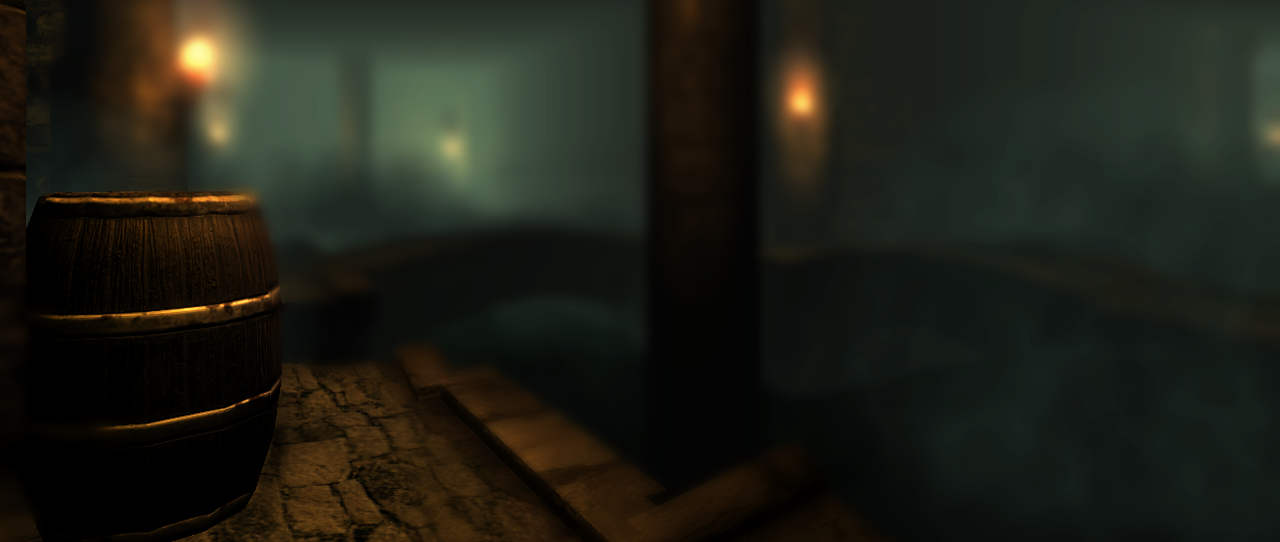
\includegraphics[scale=0.31]{C:/Users/Tasjen/Pictures/AMNESIA_SCREENS/r3.png} \\
\end{center}

Wstępując z wpół wypaloną lampą oliwną do starej rozlewni ogarnął mnie zupełny mrok. Jednak gorzej przedstawiała się sytuacja parę kroków dalej, kiedy to moim oczom ukazała się przepaść. Pomyślałem.. ślepy zaułek? - Niemożliwe. Rzucając skalny odłamek przed siebie usłyszałem wyraźnie że jakieś paręnaście metrów dalej wyrwa ta uchodzi i wraca do wysokości poziomu na którym się znajduję. Postanowiłem znaleźć jakiś sposób na przedostanie się na drugą stronę. Rozejrzałem się wokoło, żadnych lin, żadnych łańcuchów ani desek, ledwie kilka skrzynek w żaden sposób nie pozwalających przekroczyć tej zapadliny, ale zaraz... wchodząc na jedną z nich rozświetliła mi się nisza prowadząca wzdłuż korytarza. Wdrapałem się czym prędzej i ruszyłem ostrożnie przed siebie rozglądając się wokół co za miejsce mnie otacza. Jak zdążyłem dostrzec pełno było prze najróżniejszych gratów, skrzyń, głazów przerdzewiałych żeliwnych rur i gromadzącej się na posadzce wody uchodzącej drobnymi kroplami z instalacji. Głośnym tupotem zasygnalizowałem swoje dotarcie na drugą stronę, nie różniącą się niczym szczególnym, tak więc bez większego wrażenia kontynuowałem przeprawę. W komnatce obok znalazłem zawory sterujące szambem wylewającym się z dolnego poziomu kanałów. Próbując odkręcić zawór naglę usłyszałem zgrzyt, świst i zawór pękł. Aby cokolwiek z tym zrobić potrzebowałbym jakiegoś substytutu, jednak co tu takiego mogłoby mi się przydać. W przegniłej, drewnianej skrzyni udało mi się znaleźć drewnianą korbę, spróbujmy ją jakoś wykorzystać. Unosząc ją w górę, dokręcając do uszkodzonego zaworu udało mi się wytworzyć opór będący w stanie zakręcić zawór zalewający kanały. Kiedy już to zrobiłem usłyszałem czyjeś kroki. Były to silne, pewne kroki. Jak gdyby człowieka tęgiej masy lub dzikiego zwierza. Chowając się odruchowo pośród grubych rur, spojrzałem dyskretnie starając się zidentyfikować nieproszonego gościa. Po chwili komnatę zaczęła przeczesywać niespotykana nigdy wcześniej krwiożercza bestia. Twarz miała totalnie zdeformowaną przybrana w żelazną kolczugę oraz ogromny tasak niszczyła wszystko co spotkała na swej drodze. Jej ryk rozbrzmiewał po całej sali. Odruchowo ruszyłem przed siebie, nie mogłem wytrzymać stojąc dłużej jak słup soli i czekać aż blzeug\footnote{Blzeug - przybrana w żelazną kolczugę, licząca ponad 2 metry człekokształtna istota lubująca w ludzkiej krwi, zdobywając ją w bestialski sposób. Przemierza najczęściej mroczne strefy podziemi żyjąc jako samotnik. }  mnie dopadnie. Biegnąc ile sił w nogach słyszałem go jakby był tuż za moimi plecami i powoli nacinał mi kark. Jeszcze chwila, jeszcze tylko kilka metrów. Muszę wytrzymać. Przeszedłszy przez metalowy właz natychmiast go zatrzasnąłem odcinając drogę blzeugowi, jednak był on na tyle szybki, że swym szarym niczym popiół ramieniem zblokował drzwi próbując się przedostać do wodociągów. Na to nie mogłem pozwolić. Z całych sił dociskałem drzwi paraliżując ramię bestii, aż w pewnym momencie krusząc mu kończynę. Blzeug zaskwierczał, zawarczał aż w końcu się poddał. Wykorzystując to, skutecznie zamknąłem właz, blokując go od zewnętrznej strony. Zamknięcie zaworu w rozlewni otworzyło przede mną kolejną drogę, drogę w dół kanału.
 \linebreak
 \\
 \\
Przemykając po rozsmarowanej w obrzydliwościach posadzce dostrzegłem, że moja dalsza wędrówka nie obędzie się na dłuższą metę na suchym gruncie. Zacisnąłem zęby i z grymasem na licu zanurzyłem się po kolana w stęchliźnie, w śmierdzącej czadzi. Nic już gorszego nie mogło mnie tu spotkać niż dodatkowe upodlenie. Krocząc przez te odmęty, błądząc po tych ciemnościach w jednym z zakamarków trafiłem na topielca. Po krótkiej identyfikacji doszedłem o wniosku, że ciało ma ledwie 2 dni. Nieszczęśnik musiał paść ofiarą jakiś tortur, w przeciwnym wypadku zostałyby po nim tylko kości. Przy jego truchle ujrzałem kamień, podobny do tego który dostałem od konającego Zikvina. Wtem zacząłem rozważać nad tym czy mają one jakiś związek z tym, że tu jestem, z tym całym jakby uniwersum wykreowanym przez piekielne zło jakie tutaj gości. Rozglądając się dokładniej trafiłem na prototyp maszynowni, wśród której znajdował się system sterujący siłownikami pozwalającymi na unoszenie potężnych obiektów. Jednak cóż to... w owej maszynie ewidentnie brakuje zębatek. Może jest jeszcze szansa na jej uruchomienie. Według ustaleń i wstępnych obliczeń inżynierskich brakuje 3 kół zębatych $ \phi $ 20. Z pewnością, podobnie jak z kolankiem w wodociągach muszą mieć zamienniki. Nie czekając dłużej ruszyłem w poszukiwania. Godziny taplaniny się jednak opłaciły. Wkrótce miałem już komplet niezbędny do uruchomienia mechanizmu. Kiedy umiejscowiłem delikatnie ostatnią zębatkę maszyna zasyczała, zadudniła, zabuczała i nagle... poczułem zjawisko rezonansu, który po chwili zaczął powoli ustawać. Pobiegłem czym prędzej sprawdzić co się stało i nagle mym oczom ukazała się tajemne przejście, które ukryte było za jedną ze ścian kanału. Nie zastanawiając się długo udałem się w tamtą stronę powolnym krokiem rozglądając się aby czy nie zaskoczy mnie kolejna niespodzianka.   Idąc natrafiłem na rozwieszone nad głową łańcuchy ginących gdzieś wysoko w mroku. Kiedy już miałem wskoczyć na jeden z nich podążając nimi w górę, nagle zza rogu zastał mnie blzeug. Jakimś cudem musiał uwolnić się z rozlewni i pełni szału rzucił się w moją stronę. Nabrałem rozbiegu, skoczyłem, ledwie chwyciłem łańcucha, którego z zaciskiem trzymałem następnie powoli wspinając się ku górze. Pełen szału blzeug rzucał się z jednego kąta w drugi próbując w jakiś sposób naruszenie konstrukcji, jednak na moje szczęście mu się to nie udało, żegnając go ozięble w mroku dostrzegłem światło nad mą głową. Pełen entuzjazmu zmierzałem ku niemu.
\section{\textbf{Rozdział 3}}
\subsection{Posiadłość Issac'a} 
\begin{center}
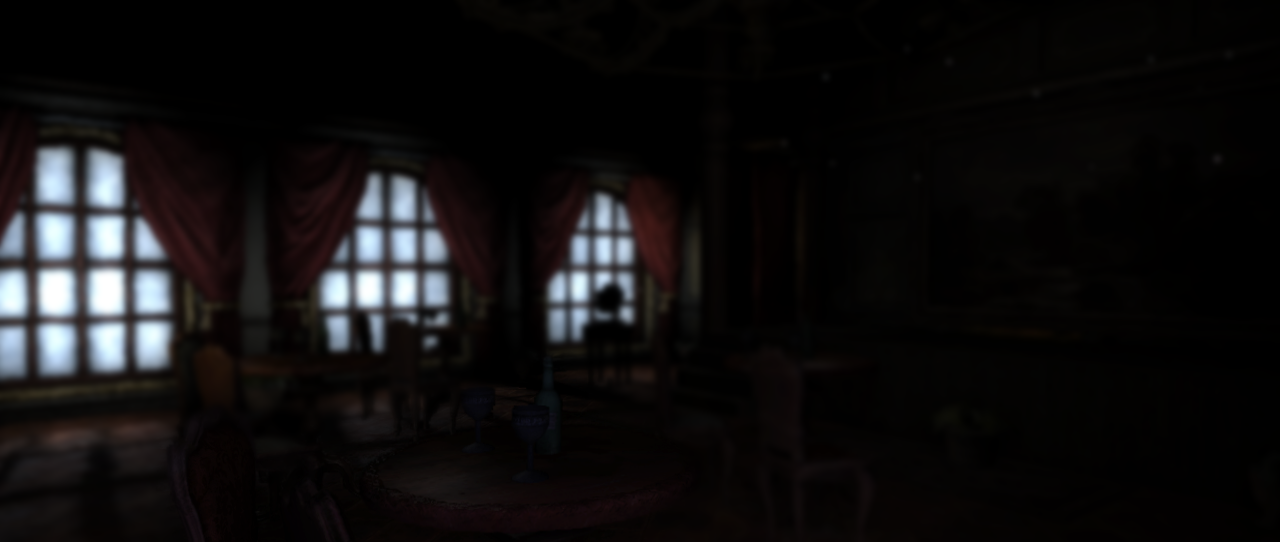
\includegraphics[scale=0.31]{C:/Users/Tasjen/Pictures/AMNESIA_SCREENS/r4.png} \\
\end{center}

Przysiadłszy chwilę, by odpocząć w odnalezionej małej, ledwie oświetlonej izebce począłem wykreślać na zakurzonej posadzce obraz mojego utraconego domu, rodziny, majątku - śmiało by twierdząc całego życia, bo kimże jest człowiek zaczynający w pewnym momencie z niczym zachowujący jedynie swój dobytek wśród głębokich wspomnień. Patrząc na ten piękny obraz zrozumiałem, że jest o co walczyć, że ta wędrówka ma szlachetny cel i nawet jeśli nie gwarantuje mi powodzenia to z pewnością zagwarantuje mi honor, który ma wszakże nieocenioną wartość. Wstając nieco zdezorientowany, uchyliłem powoli drewniane drzwi prowadząc mnie ku korytarzu jakby czyjegoś dworu. Dolewając nieco oliwy do w pół wypalonej lampy ruszyłem szukać wyjścia z tego gmachu. Posiadłość owego mościa była na tyle olbrzymia, że zajęło mi to prawie dobę szacując na podstawie położenia słońca sięgającego przez niewielkie, przybrudzone okiennice tutejszych pokoi. Z tego co udało mi się ustalić owa rezydencja była jedynie jej fragmentem. Większość drzwi, pomieszczeń i kryjówek pozostaje mi niedostępna, natomiast droga do wyjścia została zasypana stertą gruzu, cegieł i innych konstrukcji budowlanych. W jednym z salonów, bogato zastawionym ujrzałem specjalnie przygotowaną scenę, pięknie urządzone stoły dla gości z nastrojowo przygrywającą muzyką. Zakładam, że ktoś z mieszkańców miał tutaj ważną uroczystość na jego cześć i czego nie można odmówić, w kwestii gustu wyjątkowo podzielałbym uwagi tutejszych dworzan. Przemykając przez kolejne pomieszczenia trafiłem na starą bibliotekę, gromadzącą stertę ksiąg, zapisków, listów i tomy fantastycznych powieści. Przejrzawszy uważnie znajdujące się tam regały trafiłem na coś wyjątkowego. Starannie zapieczętowana kwadratowa koperta. Pomyślałbym, że to list jednakże była ona zbyt duża by przechowywała jedynie korespondencję. Otworzywszy ją delikatnie ujrzałem dużą, okrągłą, lekko chropowatą płytę winylową. Ciekaw jestem cóż za dzieło jest w niej zachowane. Wracając do salonu, w którym znajdował się odtwarzacz, poczułem wołanie żołądka. Pomyślałem, najwyższe czas na prowiant toteż priorytetem stało się uzupełnienie kalorii. Dotarłszy na miejsce, pośród zastaw w pięknie przyrządzonym stole nie zastałem nic co można byłoby przekąsić. Jednak drzwi prowadzące na zaplecze wskazywały jednoznacznie spiżarnię. Czmychnąłem szybkim krokiem jak gdyby ktoś miał mi zaraz zabrać stamtąd całe pożywienie. Przemykając pośród szafek i szukając kolejnych delikatesów począłem rozpalać w piecu, aby nieco ocieplić atmosferę. Usiadłszy na drewnianym taborecie konsumując powoli, świeżo przygotowaną pieczeń z baraniny zagryzając co kęs kawałkiem chleba dostrzegłem w pewnym momencie klapę prowadzącą w spiżarki. Wstając zaciekawiony, schylając kark dostrzegłem znajdującą się niżej chłodnie. Przeszywająca wilgoć skutecznie mnie odstraszała w tamtym kierunku jednak ciekawość była silniejsza. Idąc wgłąb trafiłem na uchodzący olej z jednej z przerwanych rur doprowadzających. Napełniłem w pół słoiczek ową mazią przypuszczając że stary odtwarzacz najprawdopodobniej będzie należało nasmarować, nim zacznie prawidłowo funkcjonować. Wychodząc chwilę później, jak gdyby zrządzenie losu, strop w chłodni pod wpływem wilgoci skruszył się zostawiając za moimi plecami stertę gruzu. Zbierając się już do wyjścia okazało się, że drzwi którymi tu wszedłem są zamknięte. Kierując się ku drugiemu wyjściu nagle usłyszałem łomot. Czyżby to znowu cadavr lub blzeug? Chowając się cichutko w kąt, pod sypiącym się przez pracę korników stole przez spiżarkę przemknął blzeug. No tak, moje przypuszczenia były co do tego jak najbardziej słuszne, trzeba jak najszybciej stąd uciekać. Wypełzając spod stołu narobiłem tylko zbędnego hałasu toteż nie mogłem zwlekać. Ile sił ruszyłem drugim wyjściem zakładając, że skoro stamtąd wyszedł to udał się w innym kierunku. Intuicja po raz kolejny mnie nie zawiodła i nim się nie obejrzałem nagle znalazłem się w holu rezydencji zamykając za sobą dyskretnie drzwi.  Wracając do salonu natknąłem się na kilka krzesiw które z pewnością powinny mi  się przydać w tych ciemnościach, oliwę natomiast zalałem do lampy. Podchodząc do odtwarzacza z gracją nasmarowałem rączkę od owego urządzenia, która w wyniku upływającego czasu była nieruchoma. Po wykonanej wstępnej konserwacji umieściłem płytę wewnątrz urządzenia, które w jednej chwili wypełniło cały dwór piękną melodią. Aż przypomniały mi się czasy kiedy to ja sam odgrywałem takie dzieła. Pomyślałem że wcale nie głupio byłoby spróbować teraz swoich sił i wykrzesać iskrę młodzieńczego talentu. Podchodząc do zakurzonego pianina zgromadzonego z resztą urządzeń w specjalnej rupieciarni w rytm muzyki zacząłem naśladować fonograf. Już dawno nie pamiętam siebie tak szczęśliwego biorąc pod uwagę ostatnie wydarzenia jakie przyszło mi pamiętać. W chwili kiedy uradowany grą nastąpił koniec melodii usłyszałem zgrzyt zamka na dole. Pobiegłem sprawdzić co się stało i oto mym oczom ukazało się przejście. Czyżby to było przejście do drugiej części owej rezydencji?
 
\subsection{Kilka stóp pod ziemią}
\begin{center}
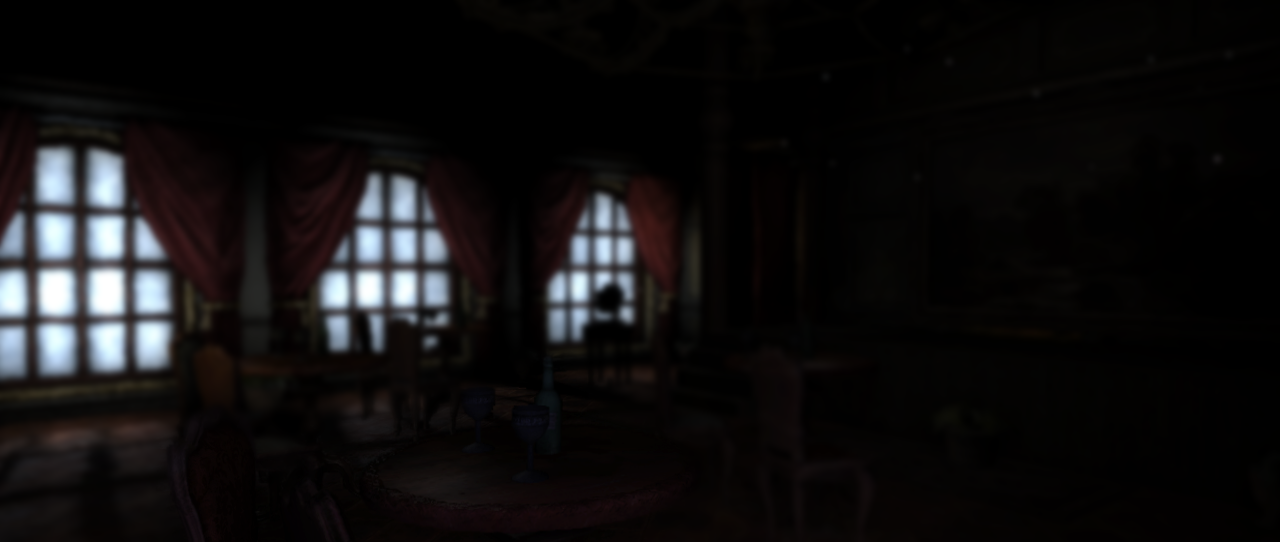
\includegraphics[scale=0.31]{C:/Users/Tasjen/Pictures/AMNESIA_SCREENS/r4.png} \\
\end{center}

Zstępując wolno, po ledwie stojącej drewnianej drabinie na dole zastał mnie, jakby na przywitanie przebrzydły smród truchła dochodzący z głębi korytarzy. Przewijając się wokół mieszczących się tam gratów, mijając ściany bogato zdobione włóknistymi pajęczymi sieciami natrafiłem na skwierczący odgłos z oddali. Nie był to przyjazny odgłos, dlatego czym prędzej uciekłem ku najbliższej, wydającej się bardziej przytulnie, skrytce. Po mijającej przez dłuższy czas ciszy, uchyliłem głowę spod opadającej drewnianej tregry, po czym ruszyłem przed siebie. W jednym z przybocznych izb odnalazłem drewnianą rączkę, pierwotnie służącą do jakiegoś mechanizmu. Zabierając ją ze sobą oraz ruszając wgłąb podziemi, nim się zorientowałem czekała już na mnie kolejna niespodzianka. Ni stąd ni zowąd wzdłuż rosnącego korytarza  
 
\section{\textbf{Rozdział 4}}
\subsection{Posiadłość Issac'a cz. II}
\begin{center}
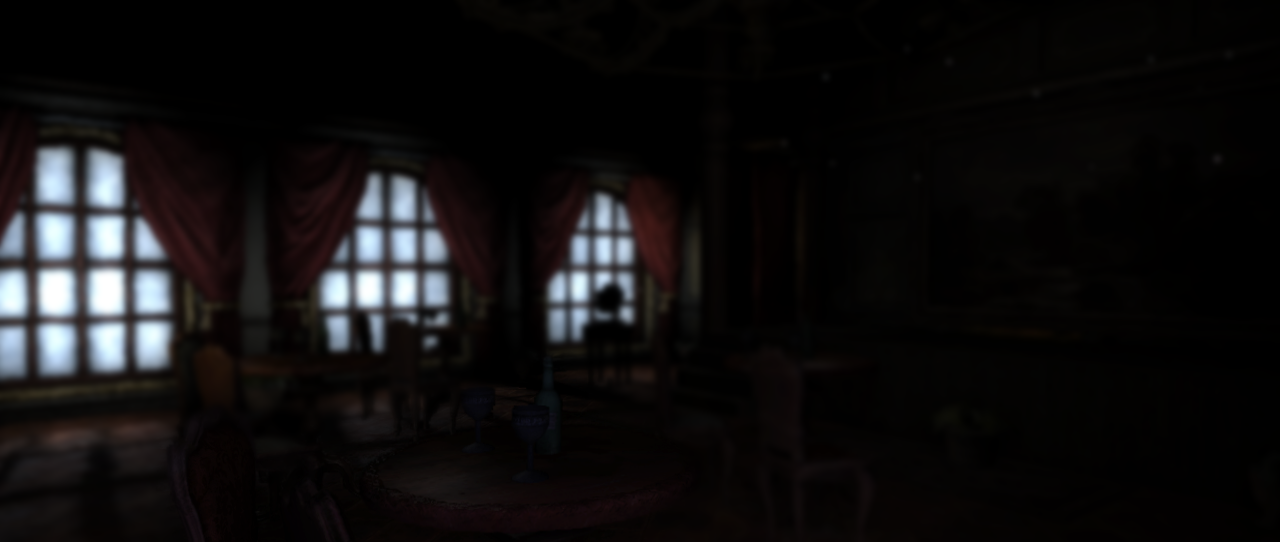
\includegraphics[scale=0.31]{C:/Users/Tasjen/Pictures/AMNESIA_SCREENS/r4.png} \\
\end{center}

Comming soon...
 
\subsection{Krematorium}
\begin{center}
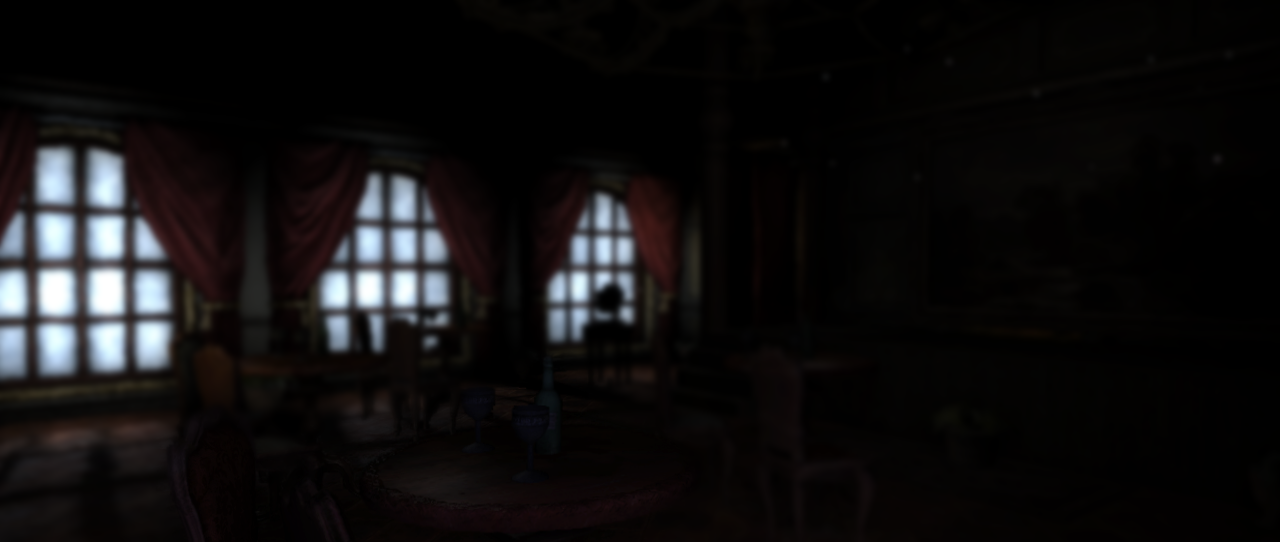
\includegraphics[scale=0.31]{C:/Users/Tasjen/Pictures/AMNESIA_SCREENS/r4.png} \\
\end{center}
 
\section{\textbf{Epilog}} 
\subsection{Koniec zła}
\begin{center}
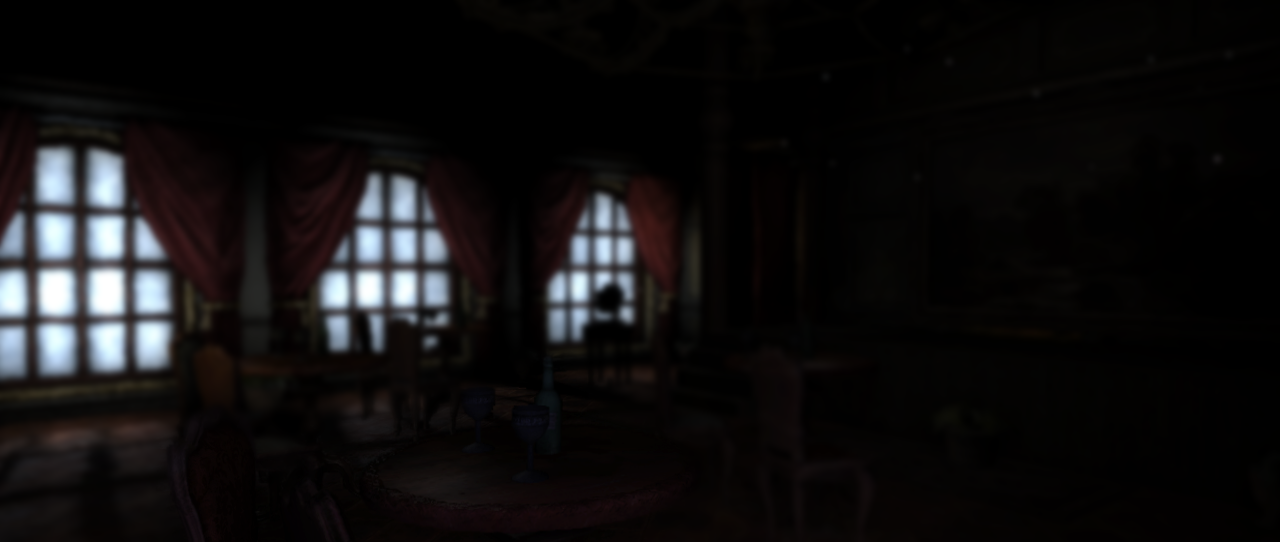
\includegraphics[scale=0.31]{C:/Users/Tasjen/Pictures/AMNESIA_SCREENS/r4.png} \\
\end{center}
 
fgfdgdfgfdg

\end{document}
